\documentclass{article}
\usepackage[T1]{fontenc}
\usepackage[utf8]{inputenc}
\usepackage[swedish]{babel}
\usepackage{amsmath, amssymb, mathtools}
\usepackage{tikz}
\usepackage{enumitem}
\usepackage{siunitx}
\usepackage{ifthen}

\usetikzlibrary{arrows}

\DeclareMathOperator\rowSums{rowSums}

\begin{document}

\section{Question \num{3.52} in Dobrow.}

\begin{center}
	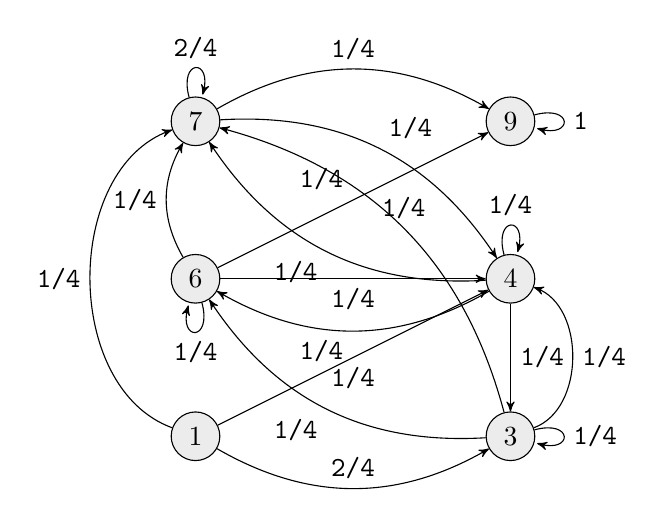
\begin{tikzpicture}[
			state/.style={ draw, circle, fill=gray!15 },
			every edge/.style={ draw, ->,>=stealth', auto, },
				]
		\foreach \x in {0,...,2}
			\foreach \y in {0,...,2} {
				\ifthenelse{\NOT 1 = \x}{
					\pgfmathtruncatemacro\label{1 + \x + 3 * \y}
					\ifthenelse{1 = \y}{\def\xp{4 - 2 * \x}}{\def\xp{2 * \x}}
					\node[state] (\label) at (\xp, 2 * \y) {\label};
					}{}
				}

		\draw (1) edge[bend right] node{\tt 2/4} (3);
		\draw (1) edge node[below] {\tt 1/4} (4);
		\draw (1) edge[bend left=70] node{\tt 1/4} (7);

		\draw (3) edge[loop right] node{\tt 1/4} (3);
		\draw (3) edge[bend right=70] node[right] {\tt 1/4} (4);
		\draw (3) edge[bend left] node{\tt 1/4} (6);
		\draw (3) edge[bend right] node[above] {\tt 1/4} (7);

		\draw (4) edge[loop above] node{\tt 1/4} (4);
		\draw (4) edge node{\tt 1/4} (3);
		\draw (4) edge[bend left] node[below left] {\tt 1/4} (6);
		\draw (4) edge[bend left] node{\tt 1/4} (7);

		\draw (6) edge[loop below] node{\tt 1/4} (6);
		\draw (6) edge node[below] {\tt 1/4} (4);
		\draw (6) edge[bend left] node{\tt 1/4} (7);
		\draw (6) edge node{\tt 1/4} (9);

		\draw (7) edge[loop above] node{\tt 2/4} (7);
		\draw (7) edge[bend left] node{\tt 1/4} (9);
		\draw (7) edge[bend left] node{\tt 1/4} (4);

		\draw (9) edge[loop right] node{\tt 1} (9);
	\end{tikzpicture}
\end{center}

The transition matrix is
\begin{equation}
	P \coloneqq \bordermatrix{~ & 1 & 3 & 4 & 6 & 7 & 9 \cr
		1 & 2/4 & 1/4 & 0 & 0 & 1/4 & 0 \cr
		3 & 0 & 1/4 & 1/4 & 1/4 & 1/4 & 0 \cr
		4 & 0 & 1/4 & 1/4 & 1/4 & 1/4 & 0 \cr
		6 & 0 & 0 & 1/4 & 1/4 & 1/4 & 1/4 \cr
		7 & 0 & 0 & 1/4 & 0 & 2/4 & 1/4 \cr
		9 & 0 & 0 & 0 & 0 & 0 & 1 \cr
		}
\end{equation}
This gives
$$ F \coloneqq (I - Q)^{-1} = \left(\begin{pmatrix}
		1 & 0 & 0 & 0 & 0 \\
		0 & 1 & 0 & 0 & 0 \\
		0 & 0 & 1 & 0 & 0 \\
		0 & 0 & 0 & 1 & 0 \\
		0 & 0 & 0 & 0 & 1 \\
\end{pmatrix} - \begin{pmatrix}
		2/4 & 1/4 & 0 & 0 & 1/4 \\
		0 & 1/4 & 1/4 & 1/4 & 1/4 \\
		0 & 1/4 & 1/4 & 1/4 & 1/4 \\
		0 & 0 & 1/4 & 1/4 & 1/4 \\
		0 & 0 & 1/4 & 0 & 2/4 \\
\end{pmatrix}\right)^{-1}
	= \begin{pmatrix}
		\cdots \\
	\end{pmatrix}
	$$
and
$$ \rowSums(F) = \bordermatrix{
	~ & ~ \cr
	1 & 9 \cr
	3 & 8 \cr
	4 & 8 \cr
	6 & 6 \cr
	7 & 6 \cr
	}
	$$
Which gives the expexted number of steps starting from each state
to first hit $9$.
Thus the answer is $9$.

\begin{enumerate}[label=(\alph*)]
	\item Find the expected length of the game.
	\item Assume that the player is on square 6.
		Find the probability that they will find themselves on square 3 before finishing the game.

		Modify $P$ to make $3$ an absorbing state and repeat the above.
\end{enumerate}

\end{document}
